\glspl{MSR} are one of six advanced reactor designs shortlisted by
the \gls{GIF} in 2001 for promising significant advances in safety,
sustainability, efficiency, and cost over existing designs in operation
today. This has attracted significant attention and resources towards
\gls{MSR} research, most noticeable by the number of start-up companies that
have emerged in recent years touting various \gls{MSR} designs. This chapter
provides a brief history of \glspl{MSR}, followed by the distinctive features
that earned the concept the label of being a Generation IV reactor. Lastly,
we present the reference specifications of the \gls{MSFR} concept studied in
this work.

\section{History}

The first \gls{MSR}, named the \gls{ARE}, dates back to the 1940s,
as part of the US Aircraft Nuclear Propulsion program
\cite{rosenthal_molten-salt_1970}; the molten salt concept was considered due
to the stability of molten salts at high temperatures and neutron radiation.
The 2.5 MW$_{\text{th}}$ reactor was built at \gls{ORNL}, where it achieved
criticality on November 1954 and generated 100 MWh over nine days
\cite{rosenthal_molten-salt_1970}. The fuel
consisted of enriched uranium in a molten salt mixture of NaF, ZrF$_4$, and
UF$_4$, and was moderated by blocks of beryllium oxide. The project ultimately
never came to fruition as the development of intercontinental ballistic
missiles effectively eliminated the need for long-range nuclear-powered
bomber aircraft.

However, the successful demonstration of the \gls{ARE} spurred further
research into adapting \glspl{MSR} for civilian power generation
\cite{rosenthal_molten-salt_1970}. One of the key findings from the
research was that breeding $^{233}$U from $^{232}$Th gave better performance
than breeding $^{239}$Pu from $^{238}$U in thermal-spectrum reactors.
Ultimately, these efforts culminated in the design, construction, and
successful operation of the \gls{MSRE}, a graphite moderated thermal
\gls{MSR}. Although the experiment did not include breeding, scientists at
\gls{ORNL} obtained a wealth of other experimental data and new insights from
the study of this reactor. The \gls{MSRE} had a
graphite-moderated design with a LiF-BeF$_2$-ZrF$_4$-UF$_4$ fuel salt mixture,
initially rated at 10 MW$_{\text{th}}$ but later restricted to 8
MW$_{\text{th}}$ due to a miscalculation of heat transfer capabilities
\cite{haubenreich_experience_1970}. 

Design of the \gls{MSRE} commenced in the summer of 1960, with construction
starting in early 1962 \cite{haubenreich_experience_1970}. The reactor
achieved zero-power criticality in June 1965, and 30 days of continuous
operation at full power in December 1966. The reactor operated at full power
for the most of the following 15 months, during which the researchers carried
out various experiments. Soon after shutdown, the $^{235}$U fuel was replaced
with $^{233}$U and in January 1969, the \gls{MSRE} became the first reactor to
run on $^{233}$U fuel. Further experiments were run, including xenon
stripping, fission product deposition, tritium behavior, and plutonium
addition studies, before the \gls{MSRE} was permanently shut down to conserve
remaining funding for other related activities \cite{macpherson_molten_1985}.

Building on the \gls{MSRE}'s hugely successful run, \gls{ORNL} proposed a
new program for the construction and operation of a demonstration reactor
based on the \gls{MSBR} concept that they had developed
\cite{macpherson_molten_1985}. The \gls{MSBR} is a thermal-spectrum, single
fluid reactor with fertile $^{232}$Th isotopes mixed directly into the FLiBe
molten salt for $^{233}$U breeding \cite{gehin_liquid_2016}. Like the
\gls{MSRE}, the \gls{MSBR} relies on continuous online reprocessing to add
fertile material and remove \gls{FP} neutron poisons. As a breeder
reactor, the doubling time (the minimum amount of time required to produce
enough fissile material to start up another \gls{MSBR}) was estimated to be
approximately 22 years. However, \gls{ORNL} failed to secure funding on two
separate occasions in 1972 and 1974; they lost out to the competing
\gls{LMFBR} program which had a head start and wider political and technical
support. Nevertheless, from a technical perspective, two independent
technology evaluation and design studies of the \gls{MSR} had ``reported
favorably on the promise of the system'' \cite{macpherson_molten_1985}.

In spite of this setback, research into \glspl{MSR} continued through the late
1970s. In 1980, \gls{ORNL} published a report describing a new \gls{MSR}
concept, called the \gls{DMSR} \cite{gehin_liquid_2016}. This design was
developed in response to the fuel reprocessing restrictions introduced by
President Ford in 1976; the \gls{DMSR} is designed to operate as a
once-through converter system without fuel reprocessing. While it is largely
fueled by 19.75 \% \gls{HALEU}, the initial core loading includes thorium to
boost its conversion ratio throughout its lifetime. It has a continuous
online feed consisting of \gls{HALEU} to maintain criticality, and denatured
$^{235}$U to keep uranium enrichment levels below nuclear non-proliferation
policy thresholds. The design also includes a gas sparging system for removing
gaseous \glspl{FP}, while noble metals naturally plate out onto the walls of
the coolant loop. A significant drawback in the \gls{MSBR} design is the
extensive neutron damage in the graphite moderator that necessitated frequent
replacement (every four years) throughout its operational lifetime. The
\gls{DMSR} avoids this issue by having a lower power density while maintaining
the overall power output of 2250 MW$_{\text{th}}$. As a result, the graphite
moderator was projected to last for the entirety of the \gls{DMSR}'s design
lifetime.

There was a concurrent program at the UK Atomic Energy Authority for the
development of a 2500 MW$_{\text{e}}$ lead-cooled
\gls{MCFR} concept \cite{smith_assessment_1974}. It is a dual fluid system,
with separate loops for the fuel salt and the blanket salt. The blanket is a
1 m-wide tank surrounding the core. The relatively harder neutron spectrum
arising from the absence of moderators and the choice of chloride over
fluoride salt favors $^{239}$Pu breeding over the thorium cycle. Some
experiments were performed to study molten salt chemistry but no reactor
prototypes were built. The UK program was eventually shut down just like its
US counterpart partly due to the successful demonstration of the Prototype
Fast Reactor which had achieved criticality in 1974.

Following a lull lasting through the late 20th century, \gls{MSR} research
picked up pace due to renewed interest initiated by the \gls{GIF} in 2001.
Today, there are numerous \gls{MSR} concepts under active development led by
various national and commercial bodies. Many differences exist between
different concepts and the only common denominator is the use of nuclear fuel
dissolved in molten salt. Table * is a non-exhaustive list of \glspl{MSR}
under development.

\section{Features}

As mentioned in the introduction section, the most significant difference
between \glspl{MSR} and other reactor concepts is the liquid fuel in
\glspl{MSR}; fissile and/or fertile material is dissolved in high temperature,
commonly eutectic mixtures of molten salts. Most \gls{MSR} designs are
circulating-fuel reactors. The primary coolant loop containing the fuel salt
transfers heat through a heat exchanger to the clean, secondary/intermediate
loop. The liquid fuel form allows for continuous online fuel reprocessing,
and the removal of gaseous \glspl{FP} via a gas sparging system.

The flexibility of \glspl{MSR} is best illustrated by the various designs
under development today. Graphite-moderated thermal-spectrum \glspl{MSR} are
typically straightforward \gls{LEU} burners, or $^{232}$Th/$^{233}$U
iso-breeders/breeders, while epithermal- and fast-spectrum \glspl{MSR} have
the additional options of operating as \gls{TRU} fuel burners or
$^{238}$U/$^{239}$Pu breeders. Breeder designs can be further categorized into
one- or two-fluid designs; two-fluid designs feature separate blanket molten
salt mixtures that contain higher proportions of fertile material than the
fuel salt mixture.

\subsection{Safety}

\glspl{MSR} are generally deemed to be safer than \glspl{LWR} due to their
reliance on natural physical phenomena for passive safety.
The most immediate and significant safety characteristic is the strong
negative temperature reactivity feedback of the fuel salt. This is due to
greater temperature-induced volumetric expansion in liquid fuel than solid
fuel. Combined with the Doppler broadening of resonance capture cross sections
present in both fuel forms, we expect to observe a smaller temperature
increase following an unprotected reactivity insertion. The overall
temperature reactivity coefficient varies widely between different \gls{MSR}
designs due to other structures, such as moderators and reflectors, present in
the core. In particular, graphite moderators tend to have slightly positive
temperature reactivity coefficients. This was notably observed in the
\gls{MSBR} concept, but the total temperature reactivity coefficient was still
relatively large and negative \cite{rykhlevskii_modeling_2019}. This
phenomenon provides a large degree of control and stability as it is always
present in an \gls{MSR} regardless of the operating conditions.

Continuous online fuel reprocessing allows operators to maintain low excess
reactivity inventories in the core as additional fuel can be added on an ad
hoc basis. Reprocessing and gas sparging systems help reduce fissile
requirements by continuously removing neutron poisons. These factors, in
addition to the strong negative temperature
reactivity coefficient, diminishes the likelihood and severity of unprotected
criticality accidents in \glspl{MSR} \cite{elsheikh_safety_2013}. In the
unlikely situation where an \gls{MSR} encounters a severe runaway reaction,
we can rely on another passive safety feature called freeze plugs. A freeze
plug is a plug of solidified salt at the bottom of the core actively cooled by
fans or other cooling systems to keep its temperature just below the freezing
point of the salt \cite{aji_experimental_2020}. When temperatures in the core
exceed a certain threshold during a dangerous transient, the freeze plug melts
and the molten salt in the core drains into a containment tank designed to
keep the salt in a subcritical configuration. This is especially easy to
achieve for
thermal-spectrum \glspl{MSR} as the absence of moderators in the containment
tank would automatically bring the multiplication factor down below unity
\cite{elsheikh_safety_2013}. \glspl{MSR} also typically have large
margin-to-boiling under nominal operating conditions so that fuel salt boiling
does not occur. Furthermore, the reactor vessel is consequently subject to
much lower stresses as \glspl{MSR} operate at near-atmospheric pressure
levels. Thus, the probability of pipe ruptures due to high pressure is low.

\glspl{MSR} may be more resilient to pump failure accidents as natural
circulation could passively sustain enough heat transfer through the heat
exchanger to remove any remaining fission and decay heat after the failure. If
natural circulation proves insufficient, the aforementioned freeze plug can
drain the salt out of the core. Decay heat in \glspl{MSR} with online
reprocessing is typically lower than that in \glspl{LWR} due to the
continuous removal of \glspl{FP}. For example, the decay heat in an \gls{MSFR}
after reaching equilibrium salt composition is approximately 3.5\% compared
to 6\% in \glspl{LWR} \cite{brovchenko_design-related_2013}.

However, there are also some safety disadvantages associated with \glspl{MSR}.
Firstly, \glspl{MSR} have smaller fractions of \glspl{DNP} in the active core
region as some of them decay in the external loop regions; this complicates
reactor control and may result in faster transients due to the decrease in
average neutron lifetime. Secondly, structural materials in the core must be
resistant to salt corrosion under high temperatures and neutron irradiation
over the lifetime of the reactor. To a lesser extent, pipes should also be
corrosion resistant to prevent pipe ruptures. Lastly, fuel salt overcooling is
a potentially dangerous accident scenario as the strong temperature
coefficient can effectively cause a large reactivity insertion. Overcooling
may also cause salt to freeze and restrict flow, thereby causing a complete
loss of flow accident.

\subsection{Other Factors}

Other factors for assessing a reactor design include sustainability,
economics, waste management, and non-proliferation.

Breeder \gls{MSR} designs easily score well in the sustainability category.
\glspl{MSR} generally have good neutron economy due to little structural
material in the core and continuous online removal of neutron poisons. Noble
metal neutron poisons also naturally plate out onto the inner walls of the
loop which are generally regions of lower neutronic importance. Both
$^{232}$Th/$^{233}$U and $^{238}$U/$^{239}$Pu fuel cycles are viable
candidates for breeding in \glspl{MSR}, with the former being more suited for
thermal reactors and the latter being more suited for fast reactors. Another
benefit of this is that some \glspl{MSR} can potentially start with an initial
core loading of $^{239}$Pu with a fast spectrum before transitioning towards
$^{233}$U fuel with a $^{232}$Th feed; this measure effectively circumvents
the issue of having insufficient $^{233}$U inventory to start up the reactor.

The $^{232}$Th/$^{233}$U fuel cycle produces significantly less \gls{TRU}
waste than the other cycles due to the smaller atomic masses of $^{232}$Th and
$^{233}$U. This reduces the overall radiotoxicity and long-term decay heat
associated with long-lived plutonium and \gls{MA} isotopes. However, there are
other radionuclides such as $^{231}$Pa, $^{229}$Th, and $^{230}$U that may
pose long-term radiological concerns. Nevertheless, this feature complements
\gls{TRU} burning in fast spectrum \glspl{MSR} to reduce overall levels
of \gls{TRU} waste going into long-term storage in nuclear waste repositories.

There are some nuclear non-proliferation concerns with the thorium fuel cycle
in \glspl{MSR}.
The main concern involves the separation of the intermediate $^{233}$Pa
isotope from the fuel salt. $^{233}$Pa decays into $^{233}$U with a half-life
of approximately 27 days and $^{233}$U is at least as potent as $^{235}$U for
nuclear weapons production. The highly radioactive $^{232}$U provides some
level of proliferation resistance but it can be sidestepped by
separating away its $^{232}$Pa precursor, which has a half-life of only 1.31
days. Strong regulatory framework and close monitoring of \glspl{MSR} would be
essential to ensure non-proliferation.

The economic prospects are uncertain at the current stage of \gls{MSR}
development but we can qualitatively list the potential impacts. Capital costs
are expected to be greater due to the need for increased corrosion resistance
and the supporting reprocessing facilities. This is in spite of the reduced
pressure constraints on the reactor pressure vessel for \glspl{MSR} resulting
from the significantly lower operating pressure. There are potential cost
savings from eliminating fuel pellet and fuel assembly fabrication. Higher
fuel utilization is achievable as neutron poisons are continuously removed
from the core via the continuous online reprocessing and gas sparging systems.
Online fuel reprocessing also minimizes reactor downtime because refuelling
can be performed at any time. The higher operating temperature results in
greater thermal efficiencies and presents new opportunities beyond
conventional electricity generation, namely industrial process heat
applications and hydrogen production.

Beyond these factors, \glspl{MSR} still require significant R\&D efforts and
engineering demonstrations for experimental validation of various components
before a full commercial model can be commissioned. Work towards creating a
safety and licensing framework for \glspl{MSR} has picked up pace only in
recent years due to the growing interest from commercial \gls{MSR} developers.

\section{Molten Salt Fast Reactor}

The \gls{MSFR} is a reference fast-spectrum \gls{MSR} concept developed
under the \gls{EVOL} and \gls{SAMOFAR} projects. The main reactor
specifications and schematic view are shown in Table \ref{table:msfr} and
Figure \ref{fig:msfr}, respectively. Developed from the \gls{MSBR}, the
\gls{MSFR} is intended to run primarily on a closed thorium fuel cycle with
continuous online fuel reprocessing. Several reasons motivated the omission of
graphite moderators from the \gls{MSFR} design. Graphite is susceptible to
long-term radiation damage and replacement is likely to be necessary during
the operating lifetime of the reactor. Graphite also has a positive
temperature coefficient of reactivity; eliminating graphite from the design
ensures a greater safety margin \cite{mathieu_thorium_2006}. While negative
temperature coefficients are attainable with very thermalized spectra,
breeding ratios deteriorated significantly due to parasitic absorption in the
large volume of graphite needed for thermalization
\cite{mathieu_thorium_2006}.
%
\begin{figure}[htb!] 
	\centering
	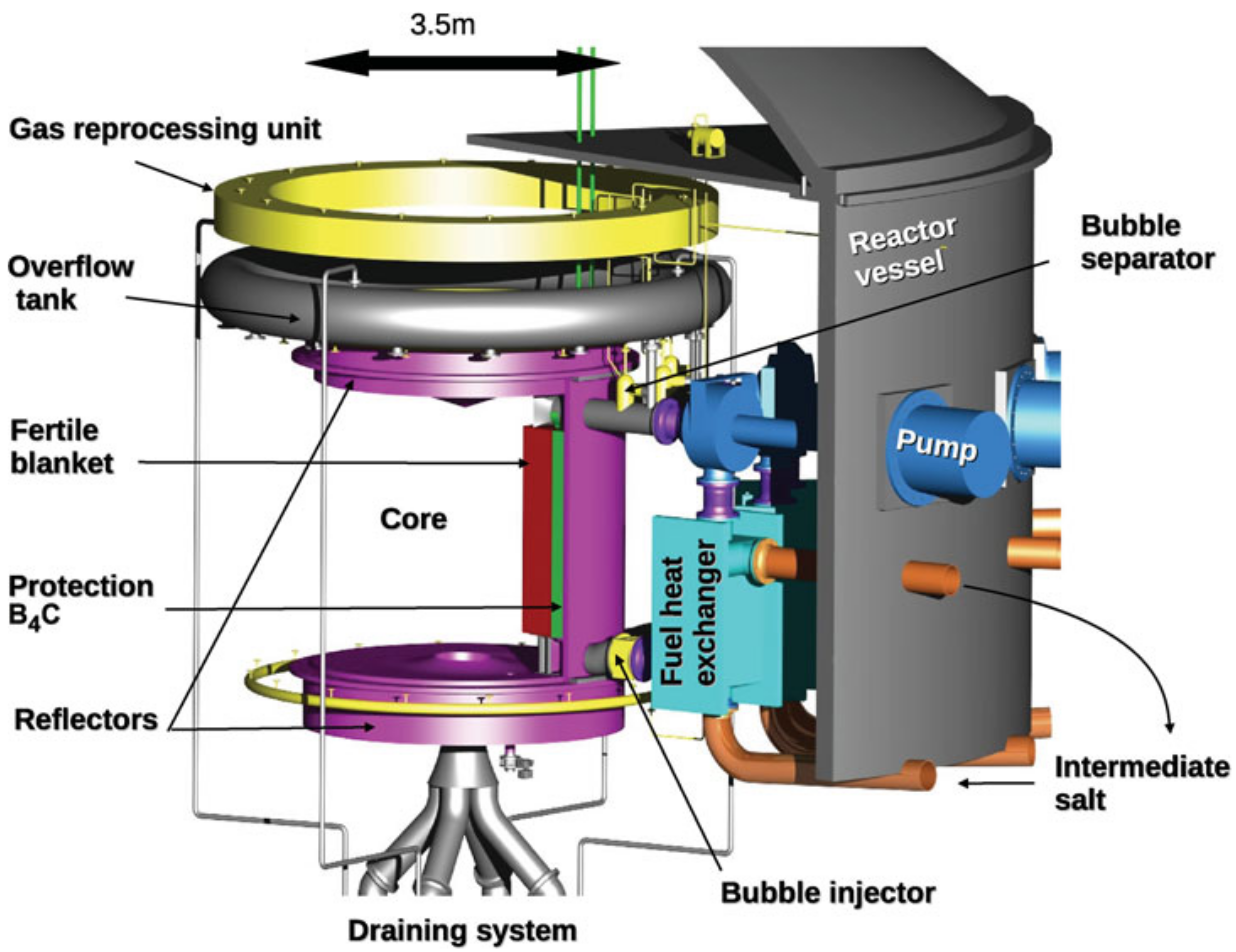
\includegraphics[width=0.6\textwidth]{MSFR}
	\caption{Schematic view of the MSFR concept \cite{serp_molten_2014}.}
	\label{fig:msfr}
\end{figure}
%
\begin{table}[htb!]
    \small
	\caption{Main specifications of the \gls{MSFR} concept
				\cite{serp_molten_2014}.}
	\centering
	\begin{tabular}{ l r }
		\hline
		Parameter & Value \\
		\hline
		Thermal/Electric output [MW$_{\text{th}}$/MW$_{\text{e}}$] & 3000 /
		1500 
		\\
		Salt volume [m$^3$] & 18 \\
		Salt fraction in core & 0.5 \\
		Number of circulation loops & 16 \\
		Nominal flow rate [kg s$^{-1}$] & 18500  \\
		Nominal circulation time [s] & 4.0 \\
		Inlet/outlet temperature [K] & 923 / 1023 \\
		Blanket volume [m$^3$] & 7.3\\
		\hline
	\end{tabular}
	\label{table:msfr}
\end{table}

In the \gls{MSFR} design, fuel salt flows upwards through a 9 m$^3$ central
core region. At the top of the core, the flow separates into sixteen smaller
external loops, each of which passes through a heat exchanger before being
pumped back into the bottom of the core. Other instrumentation are situated
along the external loop for online salt reprocessing and gas sparging. The
core is surrounded axially by nickel alloy reflectors, and radially by a
toroidal blanket tank containing fertile salt for breeding. There is a layer
of boron carbide behind the blanket tanks to protect the peripheral equipment
from excessive neutron damage. In case of severe accidents, there is an
actively cooled freeze plug at the bottom of the core that melts when
temperatures exceed a certain threshold. The fuel salt would drain into a
containment vessel designed to keep it subcritical. Reactivity control under
normal operating conditions is performed by varying pump speeds to take
advantage of the strong thermal feedback. Coupled with the fact that there is
no excess reactivity reserve due to online fuel reprocessing, there are no
control rods in the \gls{MSFR} design.

Although the \gls{MSFR} is primarily designed to operate on the thorium fuel
cycle, it can support a range of start-up fuel and feed compositions. This
versatility is particularly important for the first few \glspl{MSFR} to be
deployed due to the lack of $^{233}$U reserves required for the initial core
loading. In general, the fuel and blanket salts are approximately composed of
eutectic mixtures of 77.5\% LiF - 22.5\% AcF$_4$, where AcF$_4$ represents
actinide fluorides such as uranium, thorium, plutonium, and other \gls{TRU}
fluorides. For an initial composition consisting of $^{232}$Th and $^{233}$U,
the benchmark value for the amount of uranium for criticality under
normal operating conditions is 2.515 mol\%. However, most code verification
studies adjust the ratio of $^{232}$Th to $^{233}$U to achieve exact
criticality at a uniform temperature of 973 K; this ensures that subsequent
neutronics and safety analyses are not affected by the difference in
k$_{\text{eff}}$ values. We performed the same exercise in this thesis.

Power output of the \gls{MSFR} is rated at 3000 MW$_{\text{th}}$ and 1500
MW$_{\text{e}}$. It has a high thermal efficiency due to the high operating
temperature. \glspl{MSR} in general are not restricted by the same pressure
constraints seen in \glspl{LWR}. The inlet and outlet temperature
specifications of the fuel salt are 923 K and 1023 K, respectively. This was
motivated by the need for a minimum 50 K temperature buffer between the
operating temperatures and the melting point of the salt. The \gls{MSFR} has
heat exchangers and an intermediate coolant loop to isolate the power
conversion system from the highly radioactive fuel salt. This also serves as
a layer of containment between the radioactive material and the outside
environment. The exact composition of the intermediate coolant is still under
active study and not finalized yet.

\subsection{Model Geometry}

For this work, we used a model similar to the reference square-cylindrical
\gls{MSFR} design to benchmark our results against results published by
Fiorina et al. and Aufiero et al. The reference design is a 2-D axisymmetric
model with the sixteen individual external loops homogenized into a single
outer loop as shown in Figure \ref{fig:msfrgeom}. For the multigroup
cross sections and group constants calculations in Serpent, we extended this
2-D axisymmetric model into a 3-D model by a simple full rotation about the
central axis. The material definitions are the same as those specified in the
reference \gls{MSFR} model. Accordingly, the pump and heat exchanger regions
are assumed to be composed of 100\% fuel salt. While this may not be entirely
accurate, the exact details of the pump and heat exchanger systems are still
under active study, and this external loop region is presumed to be of little
neutronic importance due to its position behind the strong boron carbide
neutron absorber layer.
%
\begin{figure}[t!] 
	\centering
	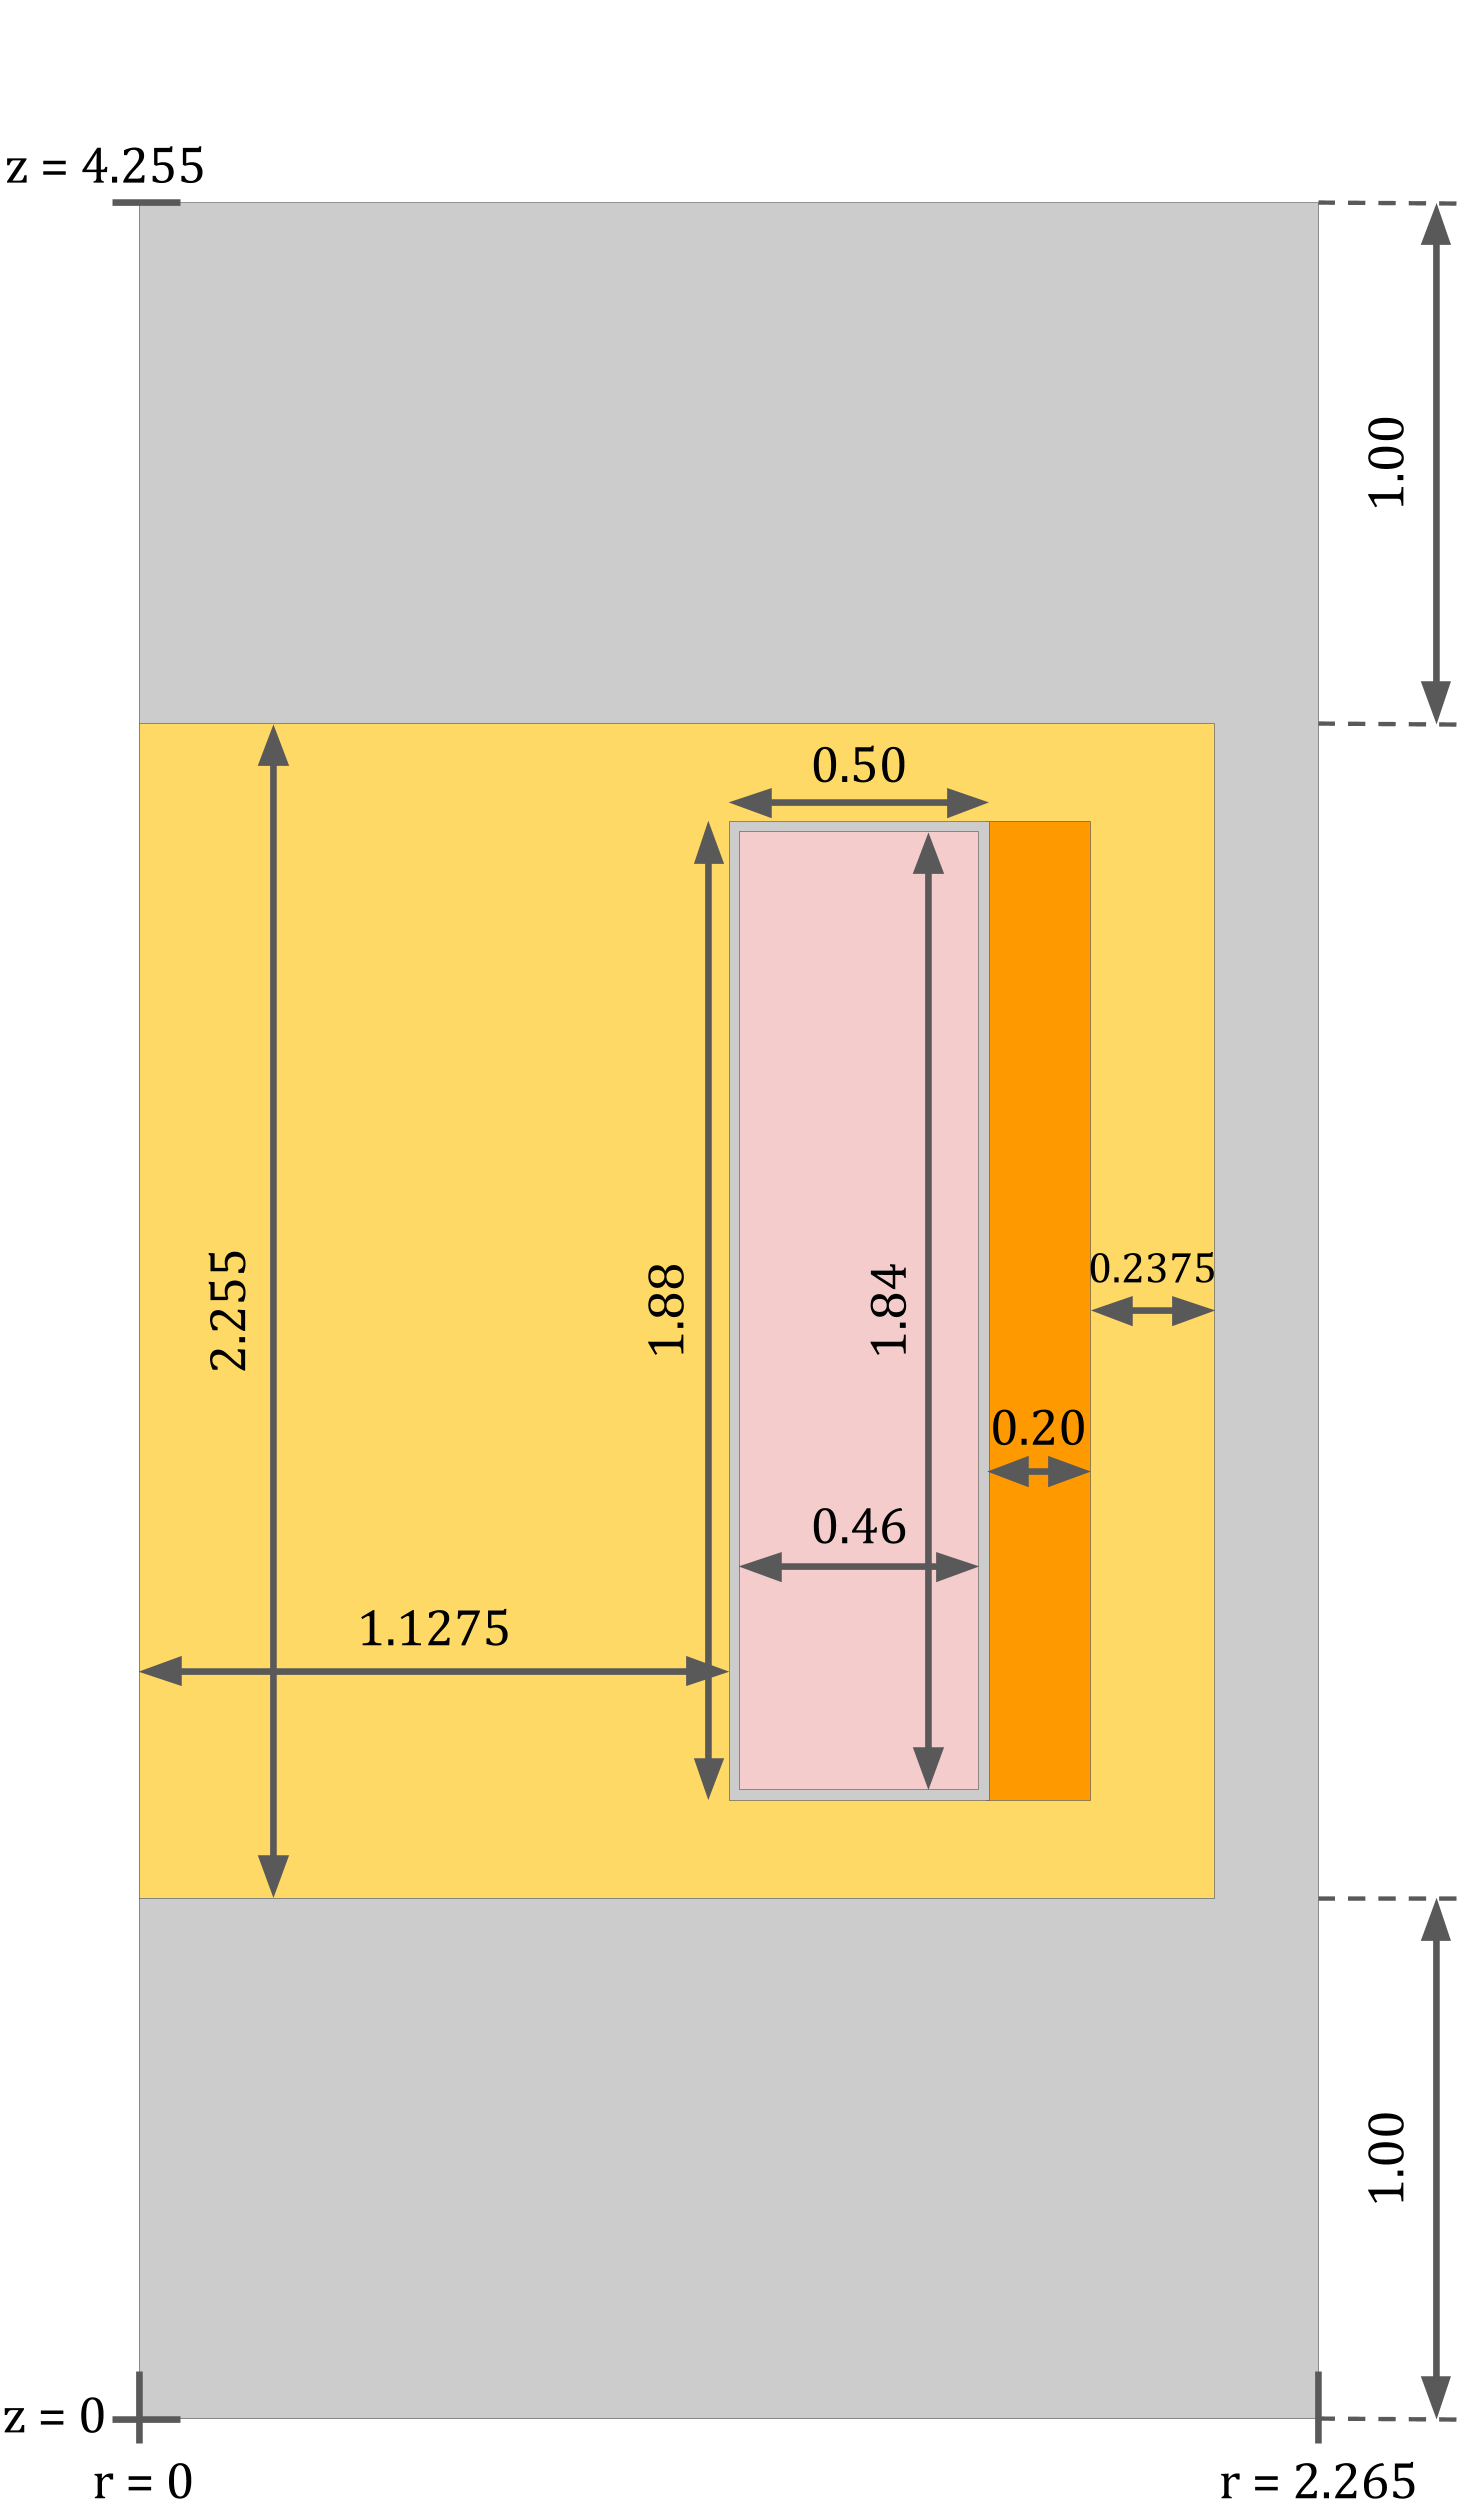
\includegraphics[width=0.5\textwidth]{msfr-geom}
	\caption{2-D axisymmetric model of the \gls{MSFR} core used for the
	simulations in Serpent. All dimensions are in meters.
	\cite{brovchenko_neutronic_2019}}
	\label{fig:msfrgeom}
\end{figure}

Although we used the exact reference model for generating group constant data
from Serpent, there are two minor differences between the \gls{MSFR} model
geometry we used in Moltres, and the Polimi/TUDelft models. The
first difference is a relative
minor change to the mesh by the exclusion of the 2 cm thick structural
material around the blanket tank that separates the fuel and blanket salts.
We removed this feature in our finite element mesh as we encountered
difficulty meshing this layer that is relatively much thinner than the rest of
the model. Any impact on the
neutron flux is expected to be minimal. Furthermore, we solved for the
temperature distribution only in the primary loop and applied homogeneous
Neumann boundary conditions for temperature on the core walls, as was done in
the Polimi/TUDelft models. Therefore, we believe the overall impact on the
results is negligible.

The second difference pertains to the modeling of the external loop. In its
current implementation, Moltres lacks sophisticated pump- and heat exchanger-
equivalents in the code. Thus, the external loop, beyond the central region of
the primary loop where most of the fissions take place, is modeled as a 1-D
pipe with a simple, point heat sink to represent the heat exchanger. Instead
of pumps, a Dirichlet boundary condition for velocity at the inlet boundaries
drives the flow in the central core region of the primary loop. All
flow-dependent variables such as temperature, \glspl{DNP},
and decay heat precursors are fully conserved as they loop around between the
two regions. As a result, this approach shares some similarities with the
geometric multiscale modeling approach by Zanetti et al.
\cite{zanetti_geometric_2015}. Future models could create a better
representation of the primary loop by implementing a whole continuous loop
with pressure increases and drops corresponding to the pumps and heat
exchangers.

\subsection{Material Specifications}

This section details the material specifications of the various reactor
components in the \gls{MSFR}.

\subsubsection{Molten Salt}

As mentioned before, the fuel and blanket salts are comprised of a 77.5\% LiF
- 22.5\% AcF$_4$ mixture. This is the reference salt composition of the
\gls{MSFR} at start-up. Typically, researchers working with the \gls{MSFR}
model calculate the exact actinide composition by varying the $^{232}$Th to
$^{233}$U ratio to obtain a $k_{\text{eff}}$ value of 1 at a uniform
temperature of 973 K. Thus, the exact actinide compositions vary depending on
the nuclear data library and neutron transport code. The exact composition
used for this work can be found in the Results chapter. We assume that the
effects of these composition variations on the reference physical properties
of the fuel and blanket salt are negligible. Table \ref{table:prip} shows
relevant physical properties of the fuel and blanket salts.
%
\begin{table}[htb!]
\small
\centering
\caption{Properties of the fuel and blanket salts LiF-AcF$_4$.}
\begin{tabular}{l l r r}
\toprule
Property & Formula & {Value at 973 K} & Validity Range\\
\midrule
Melting temperature [K] & 841 & {N/A} & 1 bar \\
Boiling temperature [K] & 1874 & {N/A} & 1 bar \\
Density, $\rho$ [kg m$^{-3}$] & $4094-0.882 \cdot (T-1008)$ & $4125$ & 893-1123 K \\
Dynamic viscosity, $\mu$ [Pa s] & $\rho \cdot 5.55 \times 10^{-8} \cdot e^{3689/T}$ & $1.015$ & 898-1121 K \\
Thermal conductivity, $k$ [W m$^{-1}$ K$^{-1}$] & $0.928+8.397 \times 10^{-5} \cdot T$ & $0.01010$ & 891-1020 K \\
Specific heat, $c_p$ [J kg$^{-1}$ K$^{-1}$] & $-1111+2.78\cdot T$ & $1594$ & 867-907 K \\
\bottomrule
\end{tabular}
\label{table:prip}
\end{table}

\subsubsection{Structural Materials}

The reflectors on the periphery of the reactor core and the blanket tank are
made of a nickel-based alloy provided from reference specifications
\cite{delpech_reactor_2009}. Table \ref{table:refl} details the compositions
of the nickel-based alloy and boron carbide absorber. The alloy has a density
of 10 g cm$^{-3}$. The material composition of the reflectors may be subject
to minor changes, but it is not a major concern as the reflectors are not
situated in regions of high neutron flux. The \gls{MSFR} also includes a 20 cm
layer of boron carbide (B$_4$C) to protect the heat exchangers and pumps from
neutron irradiation. The reference specifications indicate that natural boron
is used, which is composed of 19.8 \% $^{10}$B and 80.2 \% $^{11}$B, with an
overall density of 2.52 g cm$^{-3}$. 
%
\begin{table}[htb!]
\footnotesize
\centering
\caption{Composition (mol \%) of the nickel-based alloy used in the simulation
of the \gls{MSFR} in this work.}
\begin{tabular}{l l l l l l l l l l l l l}
\toprule
Ni & W & Cr & Mo & Fe & Ti & C & Mn & Si & Al & B & P & S \\
\midrule
79.432 & 9.976 & 8.014 & 0.736 & 0.632 & 0.295 & 0.294 & 0.257 & 0.252 & 0.052 & 0.033 & 0.023 & 0.004 \\
\bottomrule
\end{tabular}
\label{table:refl}
\end{table}
